\documentclass{article}
\usepackage{graphicx} 
\usepackage{enumitem}
\usepackage{geometry}
\usepackage{tocloft}
\usepackage{fancyhdr}
\usepackage{hyperref}

\renewcommand{\contentsname}{Table Of Content}
\renewcommand{\cftsecfont}{}
\renewcommand{\cftsubsecfont}{}
\renewcommand{\cftsubsubsecfont}{}

\pagestyle{fancy}
\fancyhf{} 
\fancyhead[C]{FinTax} 
\fancyhead[L]{}
\fancyhead[R]{}
\fancyfoot[C]{\thepage} 



\title{\textbf{SILESIAN UNIVERSITY OF TECHNOLOGY FACULTY OF AUTOMATIC CONTROL, ELECTRONICS AND COMPUTER SCIENCE - FinTax - Raport 1.
}}
\author{Kacper Szymaniak Bartłomiej Murmyłowski \\
Group: 5TI Section: 533
}

\date{19 October 2023}


\begin{document}
\thispagestyle{empty}
\newgeometry{left=5cm, right=5cm, top=3cm, bottom=3cm}   
    \maketitle
 \restoregeometry
    \newpage
\newgeometry{left=2.5cm, right=2.5cm, top=3cm, bottom=3cm}   
\fontsize{14}{16}\selectfont

\tableofcontents

    
    \newpage
    \section{Introduction}
This week, we focused on creating a graphical representation of our website - to make our work easier later on. We will have our vision at hand, rather than just in our heads, which will facilitate our work.

We began our work by creating a mockup of the website. Initially, we used the Figma application, but after encountering issues with it (such as strange graphical errors and lag), we switched to Mockflow.

We created mockups for each subpage and in two different resolutions - one for desktop browsing and one for mobile.

Why is this so important? We want the website to be responsive and perform well on various screen resolutions. According to statistics provided by Gemius Ranking, in the previous months, the majority of page views came from mobile phones, accounting for 67.94\%, while computers represented only 25.58\%.

That's why it's crucial for us to ensure that the website functions well and is responsive (as well as semantically correct). We aim to achieve responsiveness through having a mock-up of the website in advance, using appropriate technologies (e.g., Bootstrap), and writing well-structured HTML and CSS code.

Once we had our mockup ready, we fired up Photoshop and began crafting the page layout. We replaced the conceptual blocks that described the functions with actual elements, such as images, colors, and so on.

We did make a mistake, one we noticed towards the end of the process - we didn't document the padding and margins for each element thoroughly. However, we reasoned that these would likely evolve over time depending on our visual judgment.

In the subsequent part of the report, we will present this layout and its functionality.
    
    \section{Mockup}

Due to the large file size of the mockup files, we will begin by describing only the navigation bar and the footer, as these elements are consistent on every page. The remaining content will be compressed, and the entire file can be found on our GitHub repository.

\begin{figure}
    \centering
    \includegraphics[width=1\linewidth]{1.png}
    \caption{Navigation Bar - How it will look on a computer.}
    \label{fig:enter-label}
\end{figure}

We assigned a number to each element to make it easier to describe in this report.

\begin{enumerate}
    \item \textbf{Navigation Bar} - On a computer, the navigation bar will be designed to make efficient use of the wider screen real estate. Additionally, it will be sticky to the page - as you scroll down, the navbar will also move down with the page.
    \item \textbf{Logo} - The website logo will be placed at the top-left corner for brand identification.
    \item \textbf{List} - These links will be displayed horizontally across the top of the page and will typically include items like "Home," "About Us," "Services," "Contact," "Login".
\end{enumerate}

\begin{figure}[h]
    \centering
    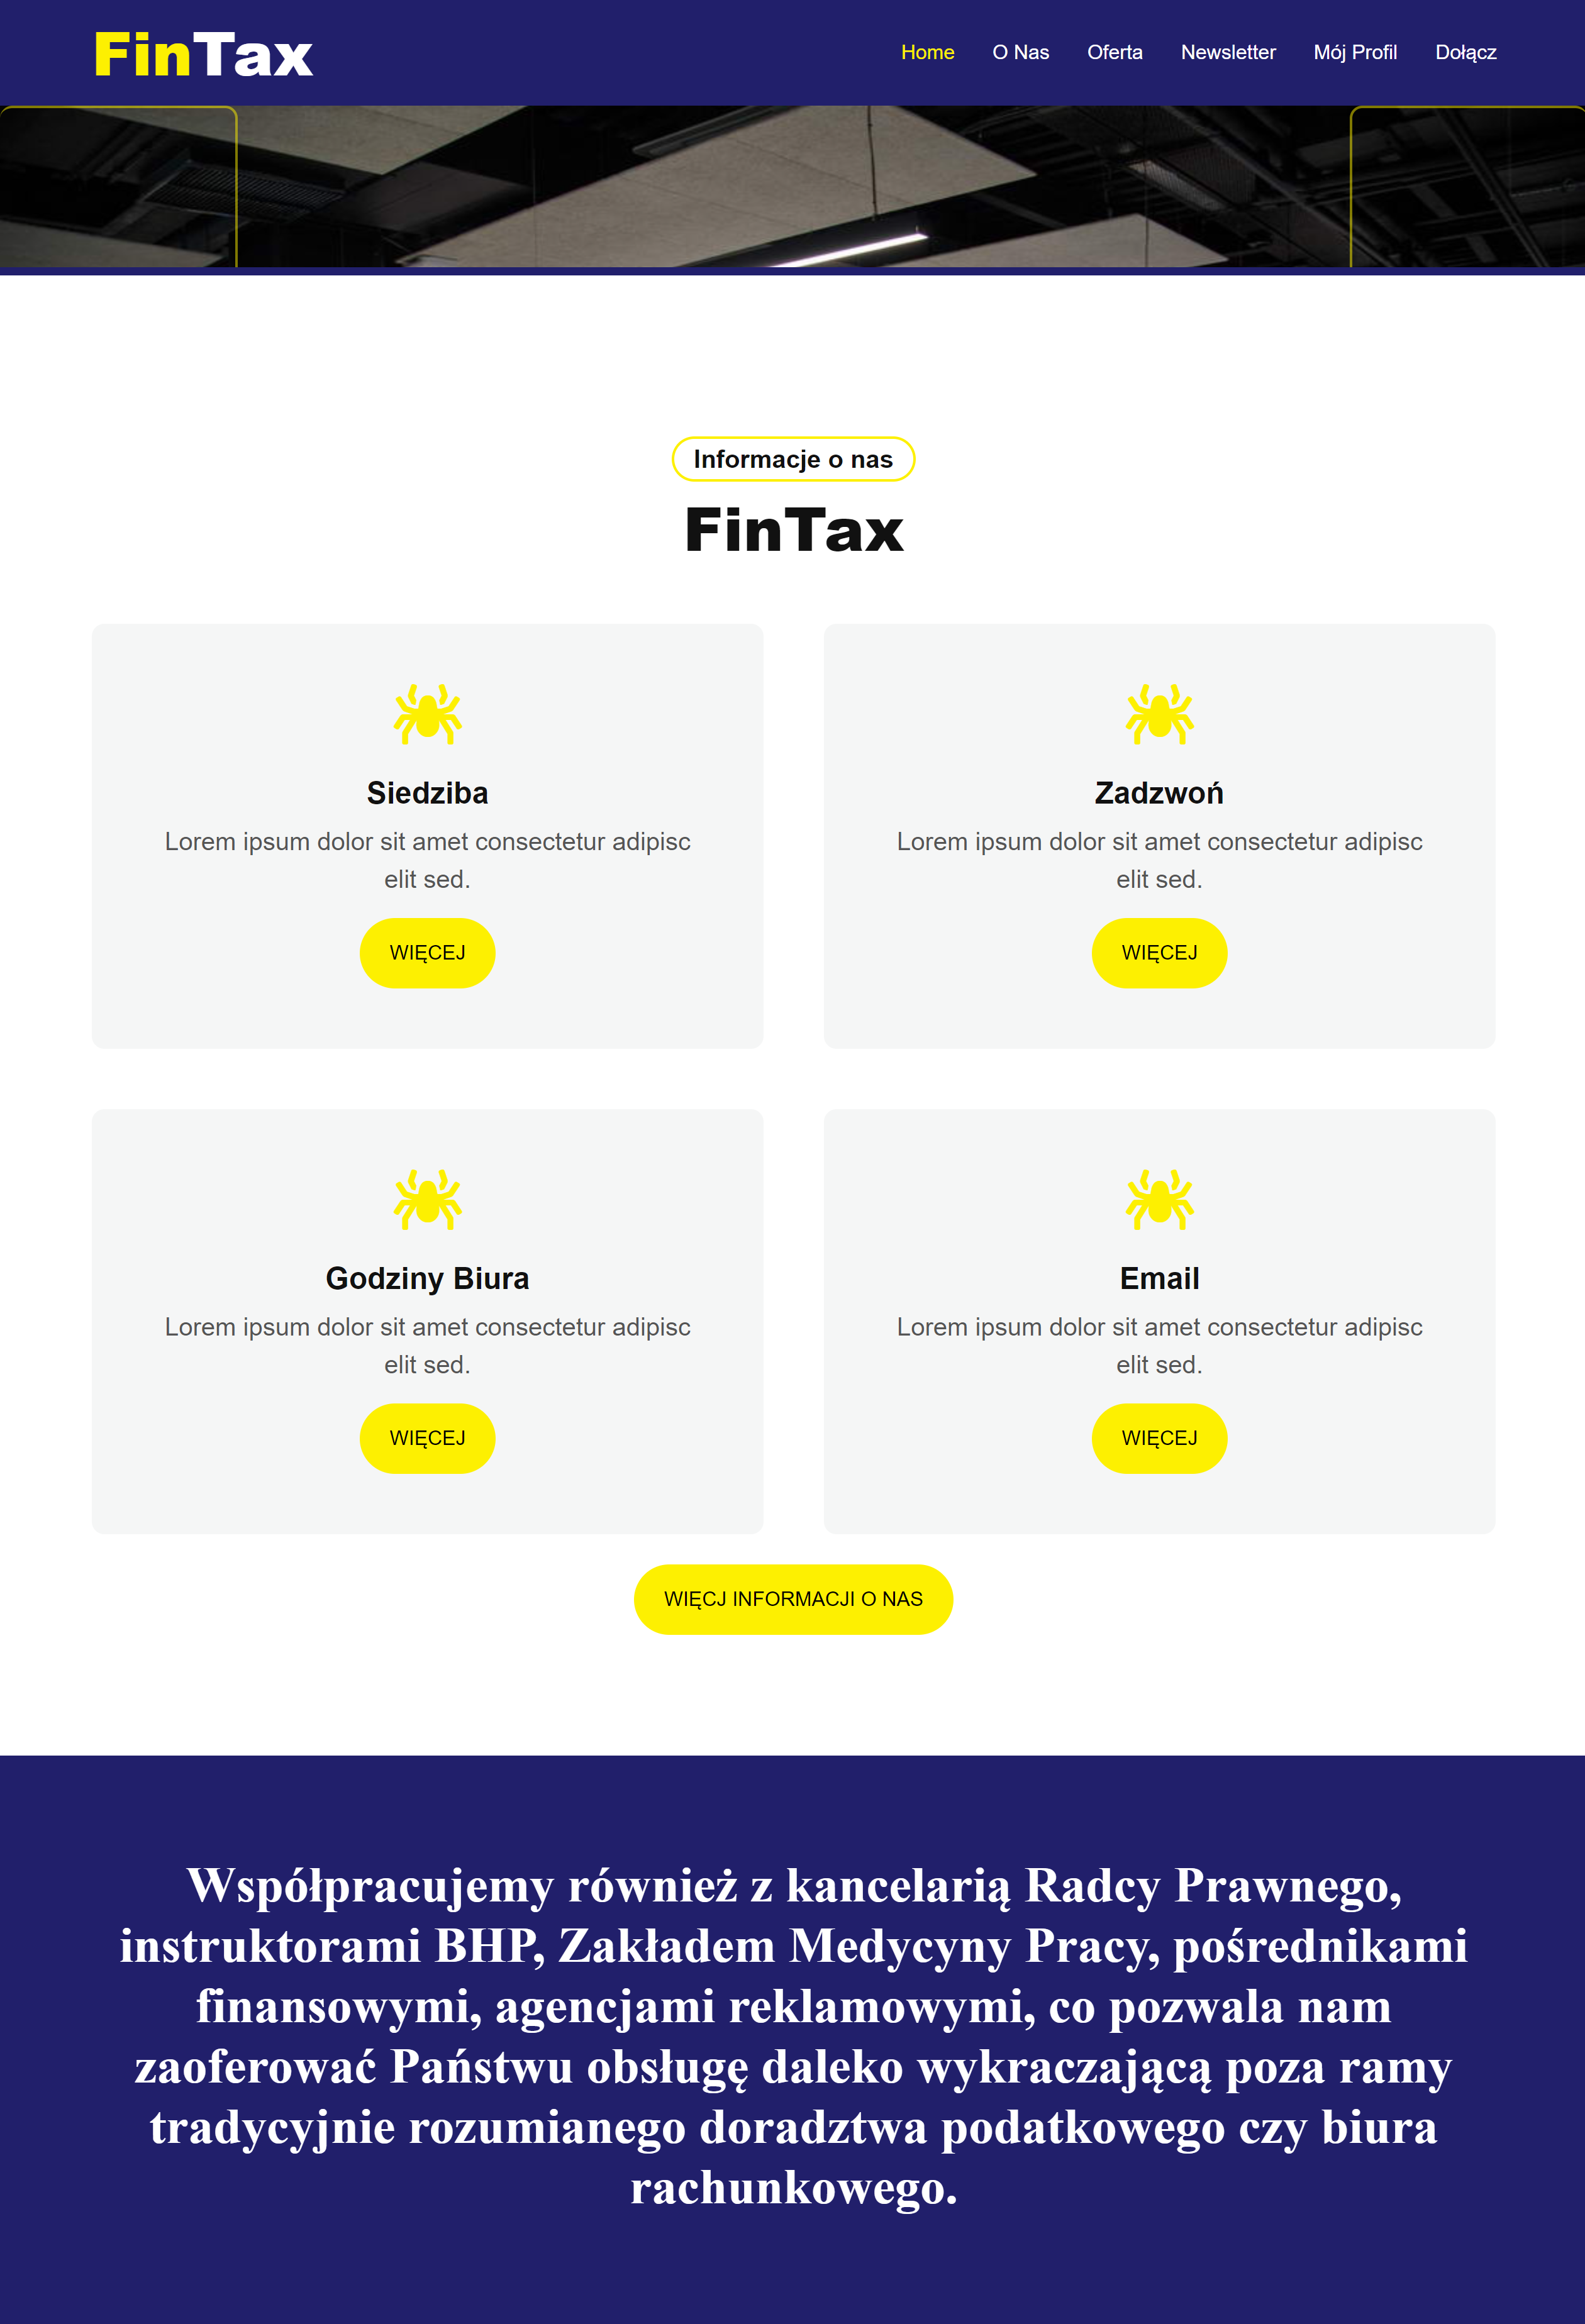
\includegraphics[width=0.75\linewidth]{2.png}
    \caption{Navigation Bar - How it will look on a mobile device.}
    \label{fig:enter-label}
\end{figure}

\begin{enumerate}
    \item \textbf{Navigation Bar} - On a mobile phone, the navigation bar will feature a responsive design to ensure it adapts to the various screen sizes and orientations of mobile devices.
    \item \textbf{Logo} -The website logo will be positioned at the top, but it will be smaller to conserve screen space.
    \item \textbf{List} - List Instead of horizontal links, there will typically be a collapsible or "hamburger" menu icon (usually represented by three horizontal lines) that, when tapped, expands to display the navigation links.
\end{enumerate}


Now, let's briefly describe how the footer looks:
\begin{figure}[h]
    \centering
    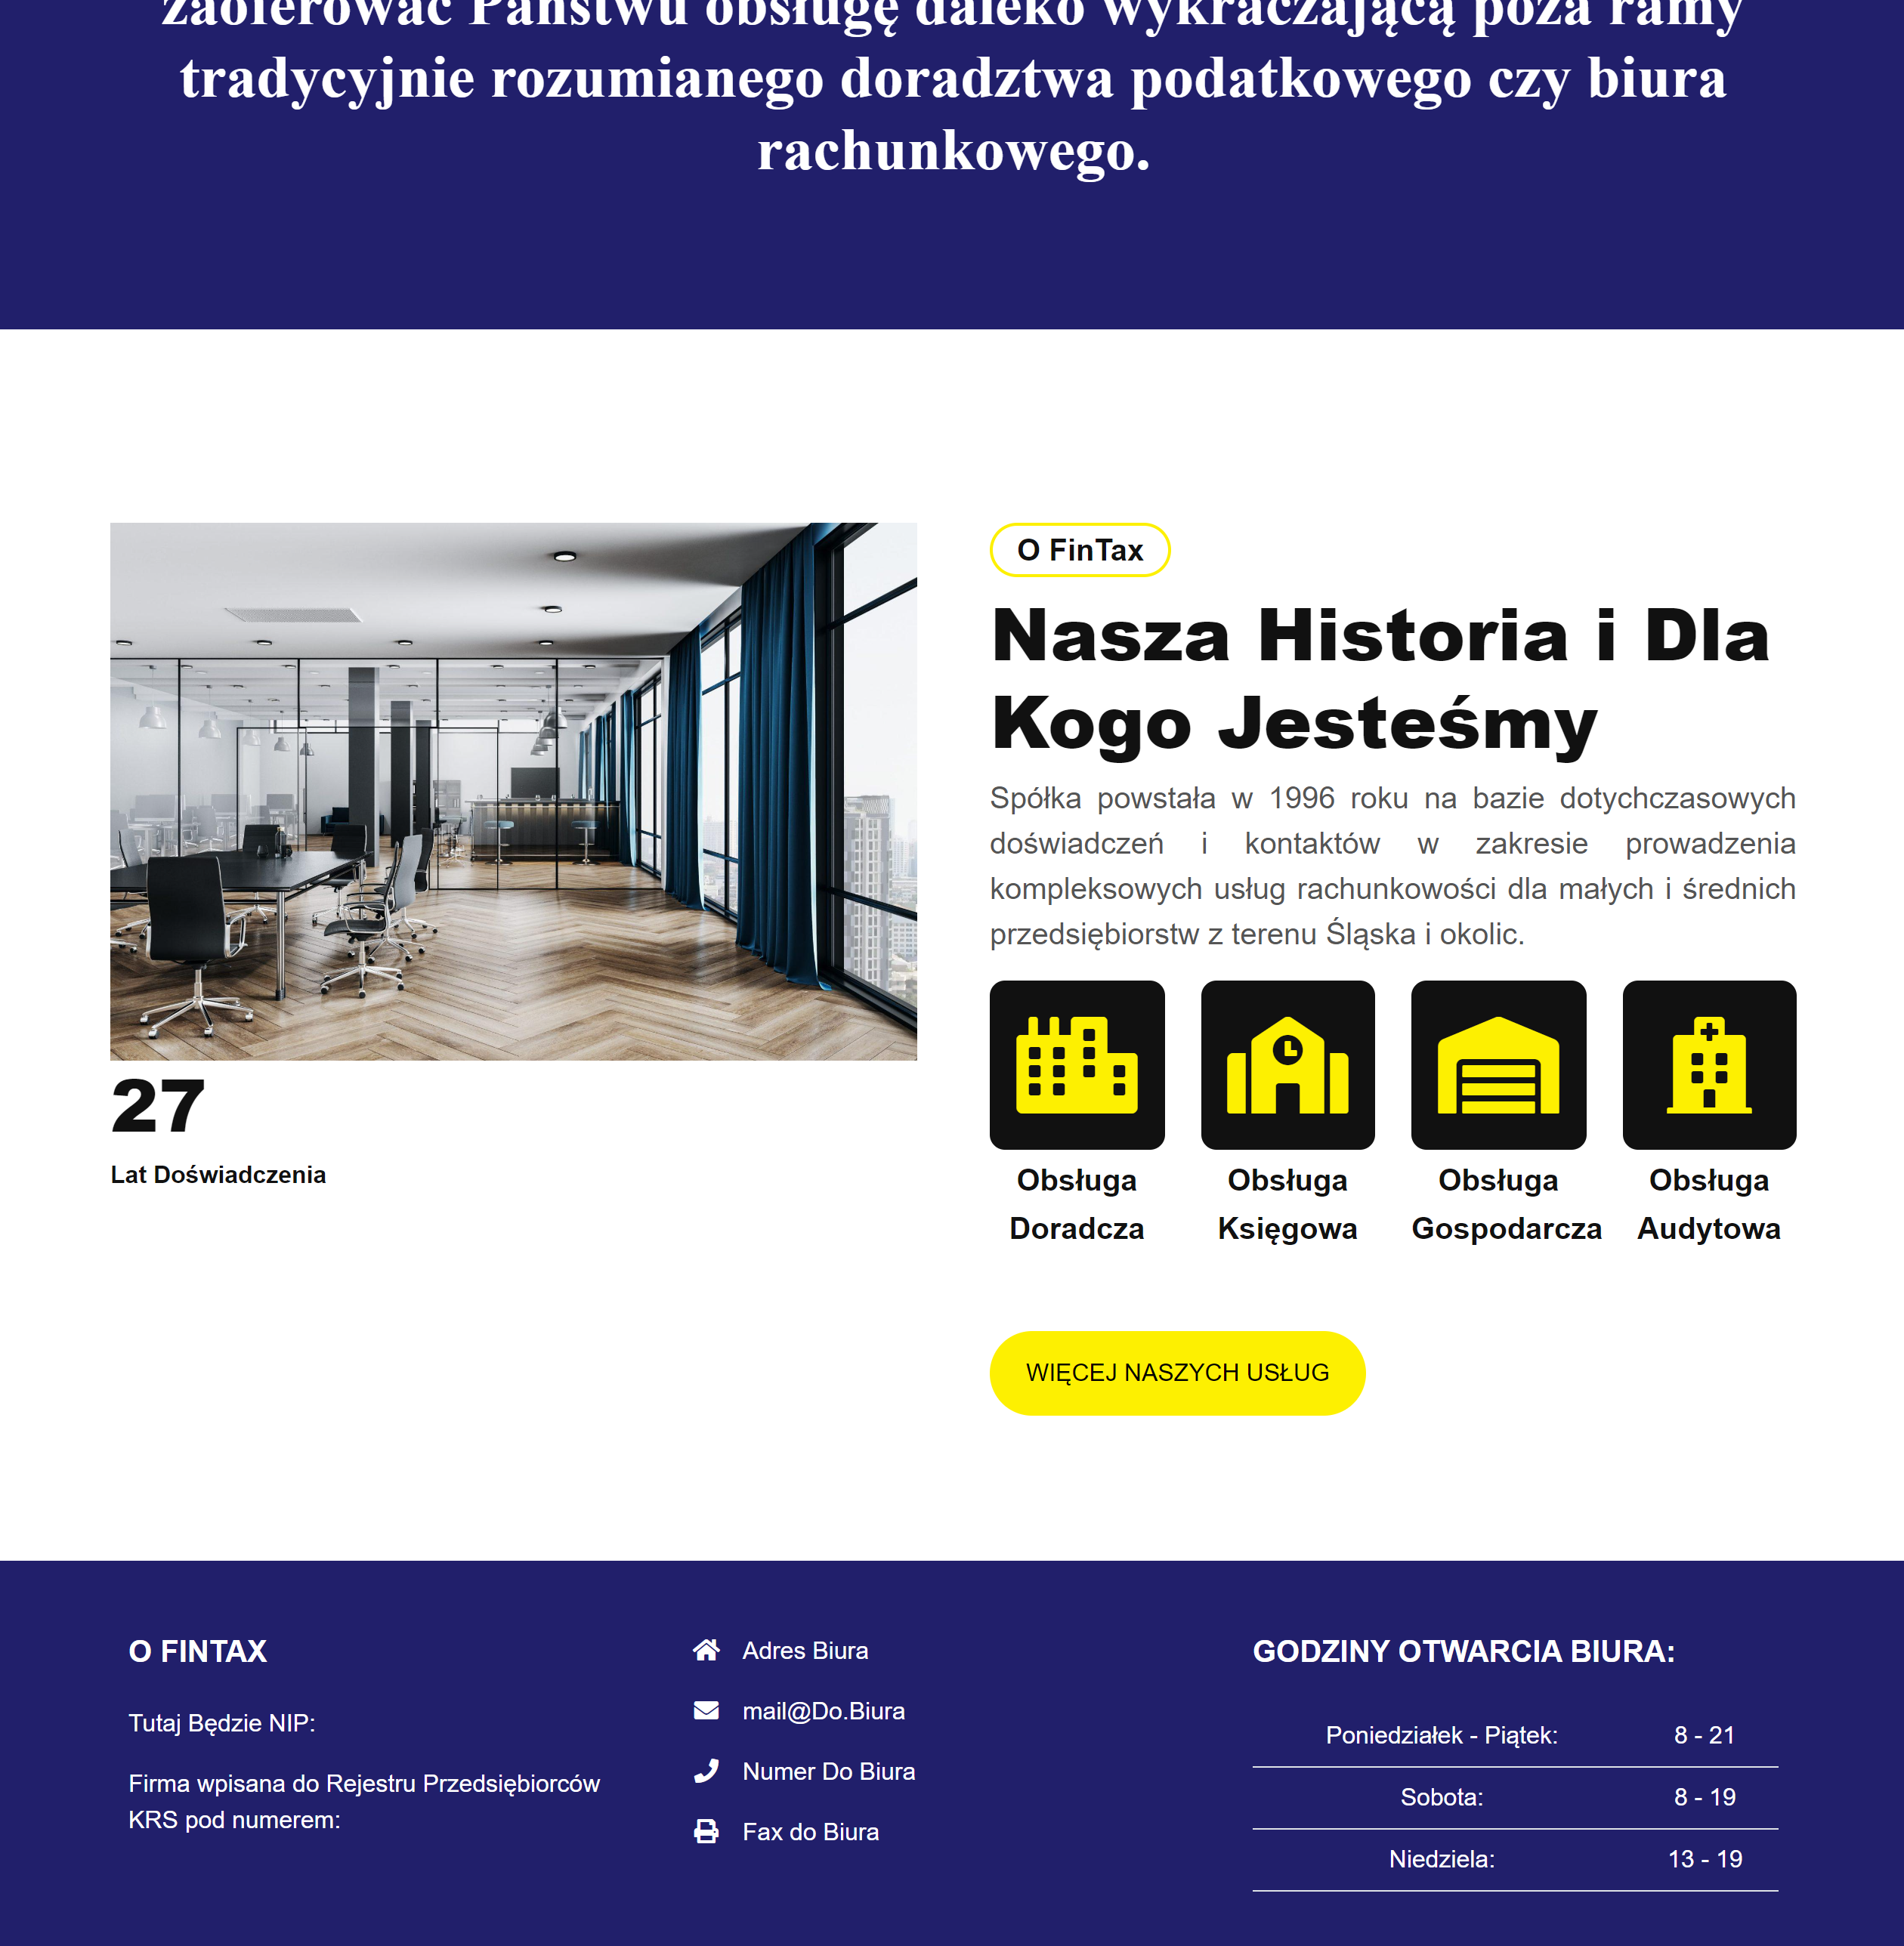
\includegraphics[width=1\linewidth]{3.png}
    \caption{Footer - How it will look on a computer.}
    \label{fig:enter-label}
\end{figure}


\begin{enumerate}
    \item \textbf{Footer} - The footer will be serving as a valuable space for providing essential information and enhancing user experience. It will be located at the very bottom of the page.
    \item \textbf{Text} - We will have text encouraging users to log in to our platform.
    \item \textbf{Text} - We will display our company's address and Tax Identification Number (NIP).
    \item \textbf{Login}  - There will be a login button.
    \item \textbf{Contact} -  We will include contact information.
\end{enumerate} 

\begin{figure}[h]
    \centering
    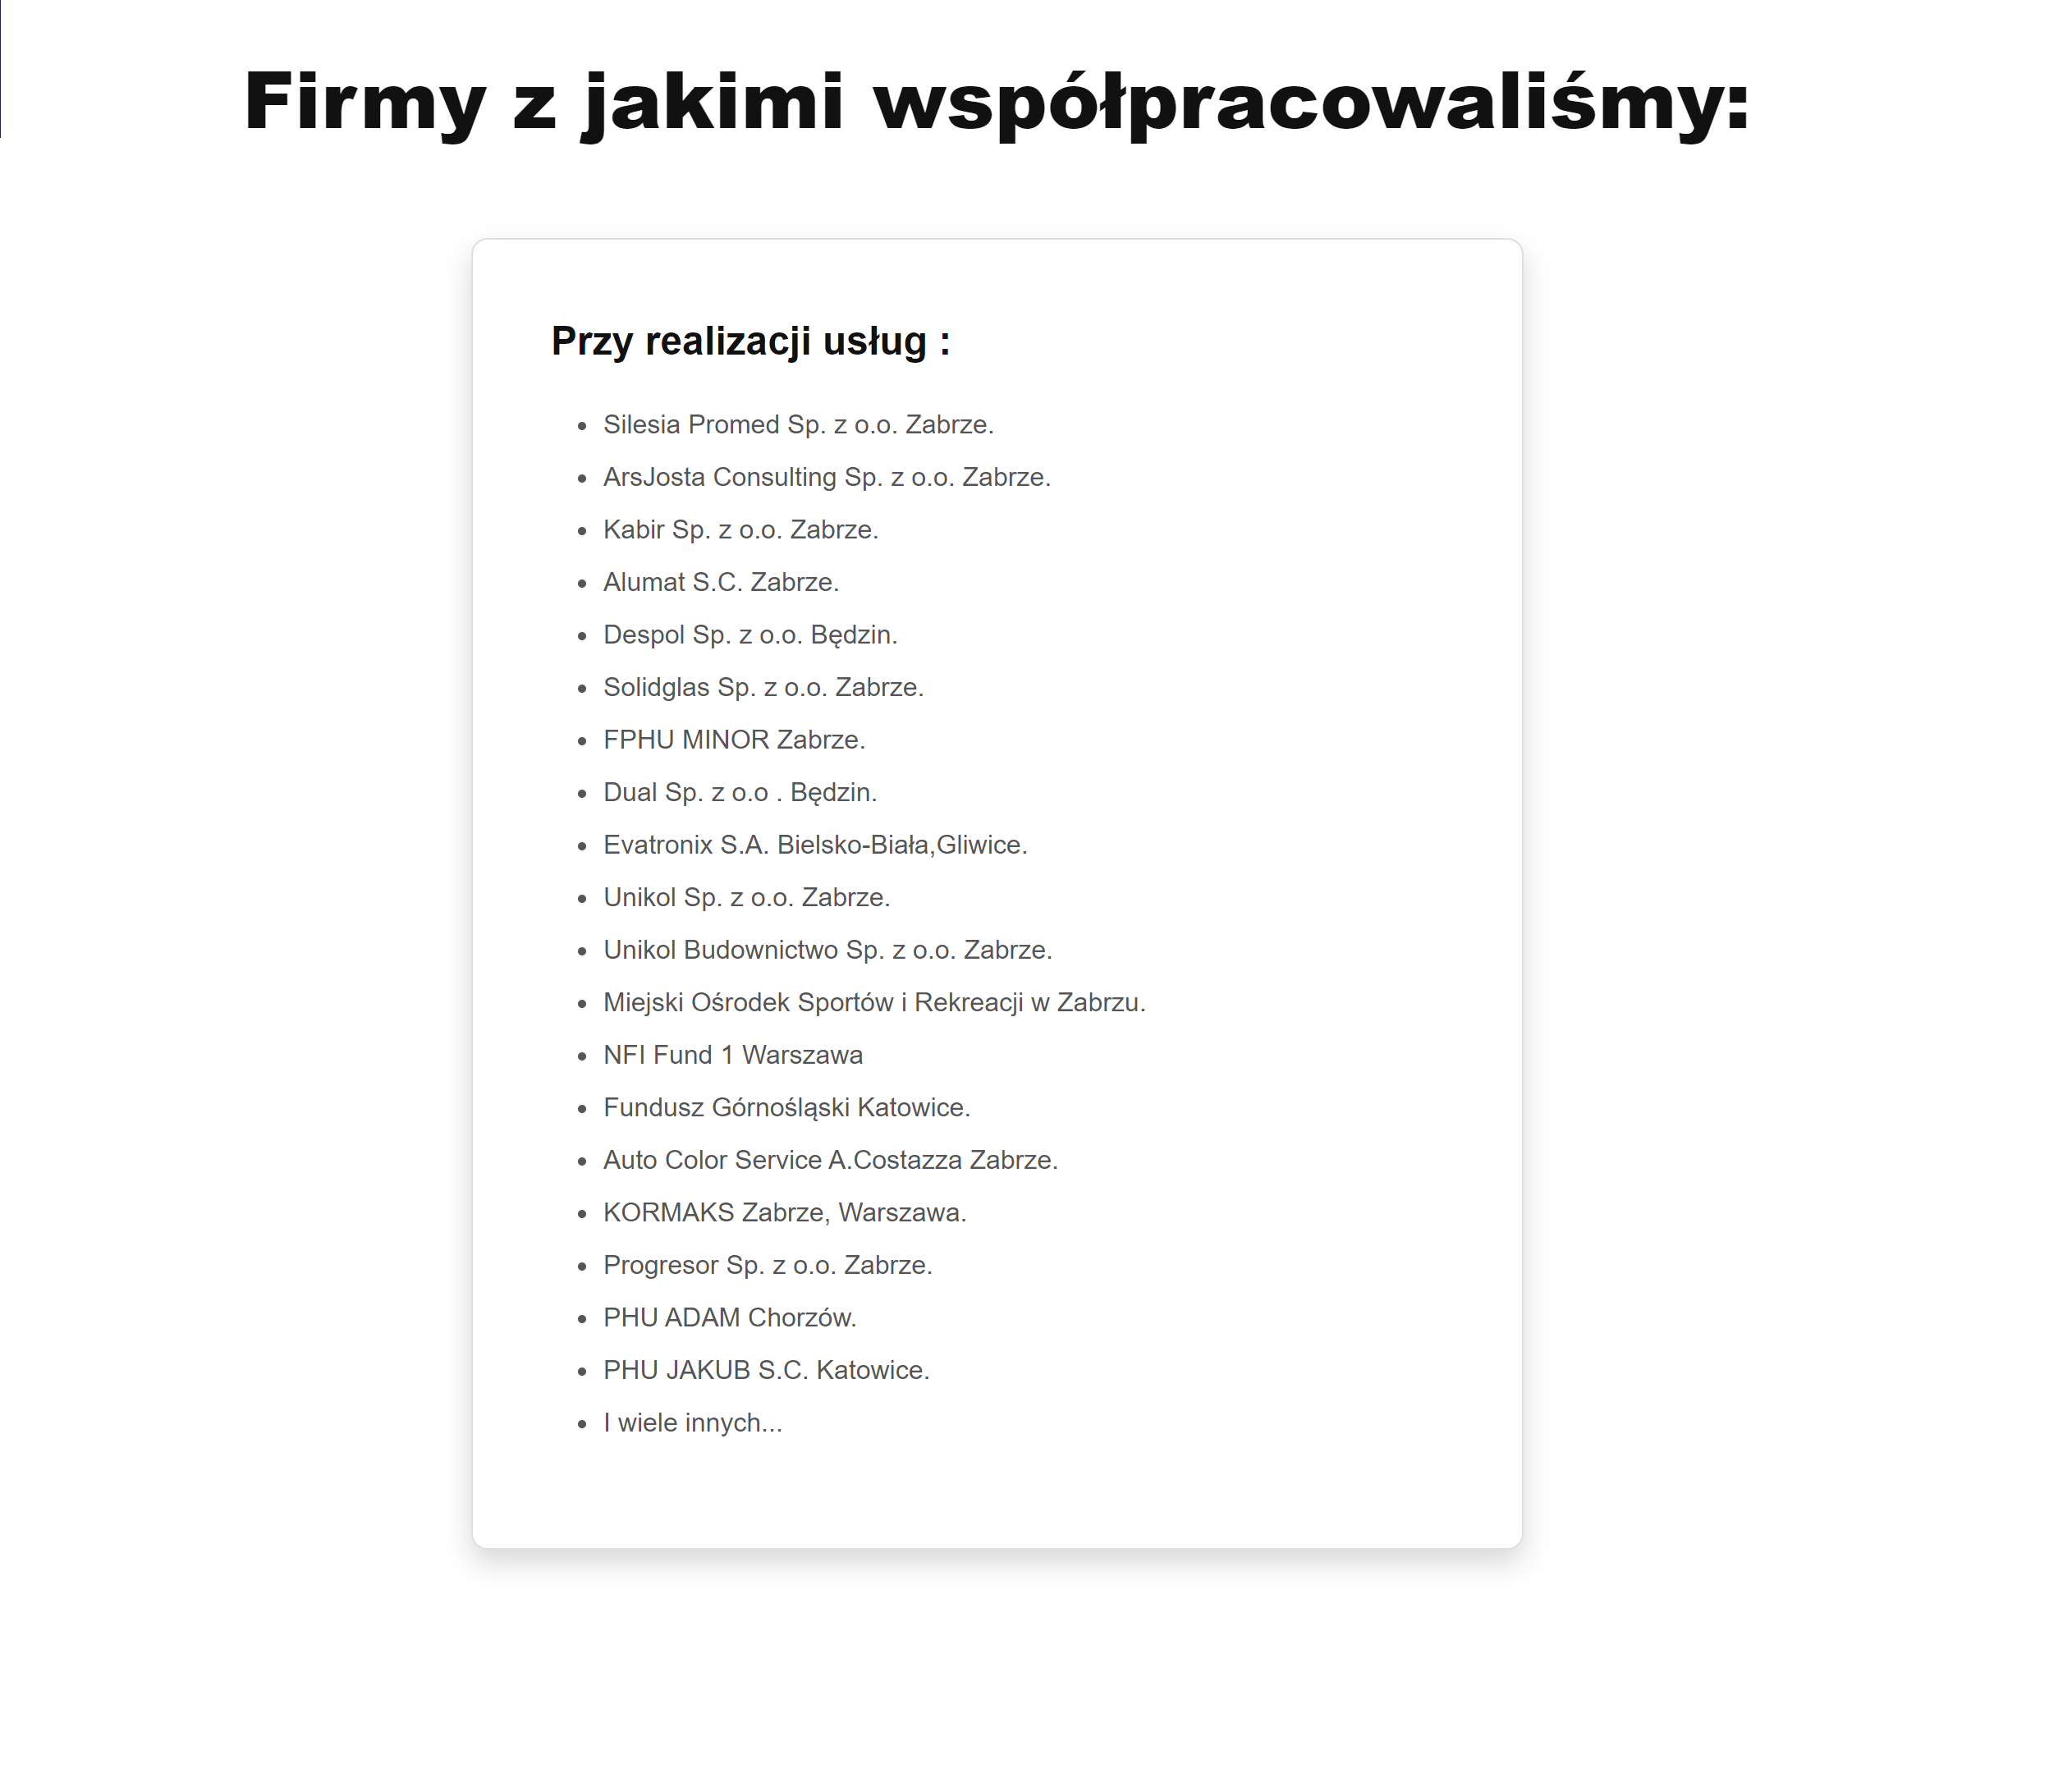
\includegraphics[width=0.5\linewidth]{4.png}
    \caption{Footer - How it will look on a mobile device.}
    \label{fig:enter-label}
\end{figure}

\begin{enumerate}
    \item \textbf{Footer} - The footer will be serving as a valuable space for providing essential information and enhancing user experience. It will be located at the very bottom of the page.
    \item \textbf{Text} - We will have text encouraging users to log in to our platform.
    \item \textbf{Login}  - There will be a login button.
    \item \textbf{Text} - We will display our company's address and Tax Identification Number (NIP).
    \item \textbf{Contact} -  We will include contact information.
\end{enumerate} 

Since we have already presented the most similar objects, we will now display the rest of our mock-up divided into subpages.
\par
\begin{itemize}
    \item \textbf{Home} \par
   As Home is the main page of our website, it must encourage our customers to trust our company. This is where the most content, images, and scripts responsible for animations will be present.
\par
   \begin{figure}[h]
    \centering
    \includegraphics[width=1\linewidth]{5.png}
    \caption{Home - How it will look on a computer.}
    \label{fig:enter-label}
\end{figure}
.
\begin{enumerate}
    \item \textbf{Gallery} - Here we have a photo gallery (with animated text related to the industry). 
    \item \textbf{Button} - On this gallery, there will be a  "Services Scope" button.
    \item \textbf{Div}  - Here, we will place three blocks side by side
    \item \textbf{Div}  - The content of these blocks includes: Office Location, Call Us, Office Hours.
    \item \textbf{Text} - Here, we plan to place the text: "COMPREHENSIVE SUPPORT AT EVERY STAGE OF YOUR COMPANY'S DEVELOPMENT."
    \item \textbf{Break} -  Here is a break - the right part of the figure is, by default, below the left part.
    \item \textbf{Text} - In these blocks, we will include things like statistics, including the number of people who have already benefited and the average duration of work on one project. We will also place a block where we will describe our company's offer.
    \item \textbf{Image} - In these blocks, we will include photos that are related to our industry and will be associated with it.
\end{enumerate} 

Since the functionality in the mobile version doesn't change significantly, only the positions of certain elements are altered; we won't describe them again. The elements will still be assigned the same numbers as mentioned above.
\par
\clearpage
   \begin{figure}[h]
    \centering
    \includegraphics[width=0.85\linewidth]{6.png}
    \caption{Home - How it will look on a mobile device.}
    \label{fig:enter-label}
\end{figure}

   \clearpage
    \item \textbf{Services} \par
   \begin{figure}[h]
    \centering
    \includegraphics[width=0.85\linewidth]{7.png}
    \caption{Services - How it will look on a Computer.}
    \label{fig:enter-label}
\end{figure}
\begin{enumerate}
    \item \textbf{Services} - We plan to showcase our services on the services plan - what the office offers 
    \item \textbf{Text} - Here, we plan to create a text in the style of 'SERVICES FOR YOUR BUSINESS.'"
    \item \textbf{Div}  - We intend to create 6 divs, each consisting of an image, bold text (h2), and a description of the respective service.

\end{enumerate} 
    Since the only change on mobile devices will be the arrangement of these 6 blocks (one below the other), we will not consider this difference here.
    
\clearpage
    \item \textbf{About Us} \par
\begin{figure}[h]
    \centering
    \includegraphics[width=0.85\linewidth]{8.png}
    \caption{About Us - How it will look on a Computer.}
    \label{fig:enter-label}
\end{figure}

\begin{enumerate}
    \item \textbf{About Us} - On this subpage, we want to display basic information about our office. 
    \item \textbf{Text} - Here, we plan to create a text in the style of 'About Us'"
    \item \textbf{Picture}  - We plan to insert a photo related to our industry here.
    \item \textbf{Text}  - Here, we will provide a brief history of our office, present statistics, and list our areas of expertise.
\end{enumerate} 
   \begin{figure}[h]
    \centering
    \includegraphics[width=0.85\linewidth]{9.png}
    \caption{About Us - How it will look on a mobile device.}
    \label{fig:enter-label}
\end{figure}

\clearpage    
    \item \textbf{Contact Us} \par


\begin{figure}[h]
    \centering
    \includegraphics[width=0.85\linewidth]{10.png}
    \caption{Contact - How it will look on a computer.}
    \label{fig:enter-label}
\end{figure}

\begin{enumerate}
    \item \textbf{Contact} - On this page, we want to include contact information for our office.
    \item \textbf{Text} - Here, we plan to create a text in the style of 'Contact Us'.
    \item \textbf{Picture}  - We plan to insert a photo related to our industry here.
    \item \textbf{Text}  - Here, we will briefly describe the ways to get in touch with our office and encourage users to log in or create an account.
    \item \textbf{Button} - This button will lead to the login page."
\end{enumerate} 
\clearpage 
\begin{figure}[h]
    \centering
    \includegraphics[width=0.85\linewidth]{11.png}
    \caption{Contact - How it will look on a mobile device.}
    \label{fig:enter-label}
\end{figure}


    

\begin{figure}[h]
    \centering
    \includegraphics[width=0.85\linewidth]{11.png}
    \caption{Contact - How it will look on a mobile device.}
    \label{fig:enter-label}
\end{figure}

\clearpage 
    \item \textbf{Login And Register} \par
    
\begin{figure}[h]
    \centering
    \includegraphics[width=0.85\linewidth]{12.png}
    \caption{Login or Register - How it will look on a computer.}
    \label{fig:enter-label}
\end{figure}

\begin{enumerate}
    \item \textbf{Login and Register} - On this page, you will have the option to log into the system. The registration page will be identical, with the exception of point 5.
    \item \textbf{Text} - Here, we plan to create a text in the style of 'Login' (or 'Register').
    \item \textbf{Input}  - Here, there will be two forms that allow you to enter an email and password.
    \item \textbf{Button}  - Here, there will be a button that will be used for logging in/registration.
    \item \textbf{Text} - Here, there will be a link for password recovery or registration.
\end{enumerate} 

Additionally, we have added a checkbox that will serve as 'remember password'.

Since this form will look the same for both login and registration on smaller screens as well as on larger ones, we won't include a screenshot of how it would appear here.\par 

    \item \textbf{Client And Admin View} \par

\begin{figure}[h]
    \centering
    \includegraphics[width=0.85\linewidth]{13.png}
    \caption{Client View - How it will look on a computer and mobile devices.}
    \label{fig:enter-label}
\end{figure}

\begin{enumerate}
    \item \textbf{Client View} - We want to build a system where a logged-in customer can enter their phone number, email, alternative contact method, preferred contact times, etc.
    \item \textbf{Text} - Here, we plan to create a text in the style of "Login".
    \item \textbf{Input}  - Here, there will be two forms that allow you to enter an email and phone number contact.
    \item \textbf{Calendar} - Here, the client will be able to select a date (day, month, time) when they can have a conversation with our consultant.
    \item \textbf{Input} - Here, the client will be able to include a message to us.
     \item \textbf{Input} - Here, there will be a button that will be used for sending a message.
\end{enumerate} 

\begin{figure}[h]
    \centering
    \includegraphics[width=0.9\linewidth]{14.png}
    \caption{Admin View - How it will look on a computer and mobile devices.}
    \label{fig:enter-label}
\end{figure}

\begin{enumerate}
    \item \textbf{Admin View} -For administrators, we want to build a system where they can check customers, their contact information, and when they can get in touch with them.
    \item \textbf{Text} - Here, we plan to create a text in the style of "Data".
    \item \textbf{Output}  - Here, there will be contact information for the customer.
    \item \textbf{Text} - Here, we will have a message from the customer and when they would prefer to be contacted.
     \item \textbf{Input} - Here, the admin could write their notes about the customer.
     \item \textbf{Button} - Here, there will be a button that will be used for saving a notes.
     \item \textbf{CheckBox} - Here, there will be a checkbox that serves to confirm contacting the customer. This will require double confirmation. Once confirmed, using the button in point 5 will remove the customer from the 'to contact' list.
\end{enumerate} 
    
\end{itemize}

    
    
\end{document}


